\subsubsection{Clean Architecture}
As already introduced, each part of our system will use the Clean Architecture, proposed by Robert C. Martin. We apply this architecture both on the mobile application and in the Application Server.

\begin{figure}[H]
\centering
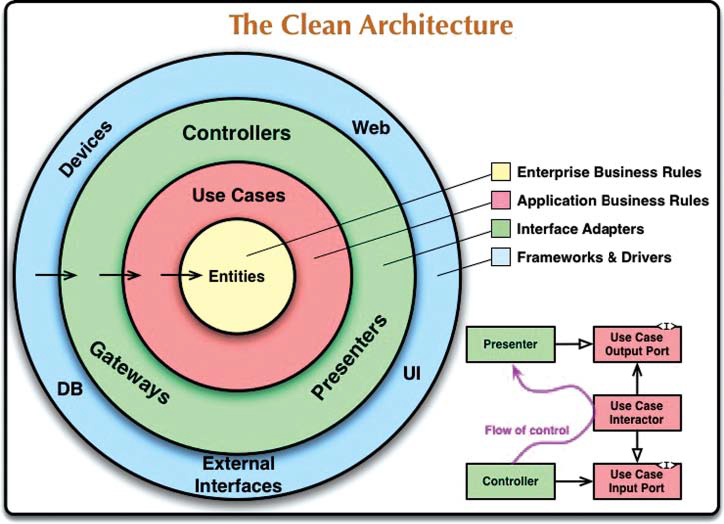
\includegraphics[width=.7\textwidth]{Images/cleanArchi.pdf}
\caption{\label{fig:cleanArchi} Clean Architecture \cite{clean} p. 203}
\end{figure}

\paragraph{Dependency Rule}
"The concentric circles in Figure \ref{fig:cleanArchi} represent different areas of software. In general, the further in you go, the higher level the software becomes. The outer circles are mechanisms. The inner circles are policies.
The overriding rule that makes this architecture work is the Dependency Rule:
\textit{Source code dependencies must point only inward, toward higher-level policies.}
Nothing in an inner circle can know anything at all about something in an outer circle. In particular, the name of something declared in an outer circle must not be mentioned by the code in an inner circle. That includes functions, classes, variables, or any other named software entity." \cite{clean}

\paragraph{Entities}
"Entities encapsulate enterprise-wide Critical Business Rules. An entity can be an object with methods, or it can be a set of data structures and functions. It doesn’t matter so long as the entities are the business objects of the application. They are the least likely to change when something external changes. For example, you would not expect these objects to be affected by a change to page navigation or security. No operational change to any particular application should affect the entity layer." \cite{clean}

\paragraph{Use Cases}
"The software in the use cases layer contains application-specific business rules. It encapsulates and implements all of the use cases of the system. These use cases orchestrate the flow of data to and from the entities, and direct those entities to use their Critical Business Rules to achieve the goals of the use case.
We do not expect changes in this layer to affect the entities. We also do not expect this layer to be affected by changes to externalities such as the database, the UI, or any of the common frameworks. The use cases layer is isolated from such concerns.
We do, however, expect that changes to the operation of the application will affect the use cases and, therefore, the software in this layer. If the details of a use case change, then some code in this layer will certainly be affected." \cite{clean}

\paragraph{Interface Adapters}
"The software in the interface adapters layer is a set of adapters that convert data from the format most convenient for the use cases and entities, to the format most convenient for some external agency such as the database or
the web. The presenters, views, and controllers all belong in the interface adapters layer. The models are likely just data structures that are passed from the controllers to the use cases, and then back from the use cases to the presenters and views." \cite{clean}

\paragraph{Adantages of Clean architecture}
Following are some reasons wh a good architectural pattern for our system:
\begin{itemize}
  \item All business logic is in a use case, so it’s easy to find and not duplicated anywhere else
  \item Good monolith with clear use cases that you can split in microservices later on

\end{itemize}


\subsubsection{REST}
The communication between the mobile application and the microservice will be done via HTTP requests following REST principles. REST (Representation State Transfer) is an architectural style for communication based on strict use of HTTP request types. One of the most important REST principles is that the interaction between the client and server is stateless between requests. Each request from the client to the server must contain all of the information necessary to understand the request. The client wouldn’t notice if the server were to be restarted at any point between the requests.


\subsection{Other design decisions}
Here we describe the frameworks and languages hat should be used to produca a state-of-art application.

\paragraph{Flutter}


\paragraph{Node.js}
To build a

\paragraph{MongoDB}
MongoDB is a noSQL database. It represents the data as a collection of documents rather than tables related by foreign keys. Those documents are collected in collections and can have different schemas. We choose to use MongoDB because it's so well intergrated with Node.js, because there are very useful libraries such as Mongoose whick make easier to communicate with the DB. Document-based data storage is the main aim of using a non-structured database like NoSQL. MongoDB is a distributed database which allows ad-hoc queries, real-time integration, and indexing efficient.
